\section{Theorie}
\label{sec:Theorie}
\subsection{Ziel}
 In diesem Versuch soll die effektive Masse von Elektronen in Halbleitern mit Hilfe des Faraday-Effekts bestimmt werden.
\subsection{Die effektive Masse}
 Mittels Energiebändern, wie in Abbildung \ref{fig:Energiebänder} zu sehen, lassen sich verschiedene physikalische Effekte
 von Kristallen beschreiben.
 \begin{figure}[H]
 \center
 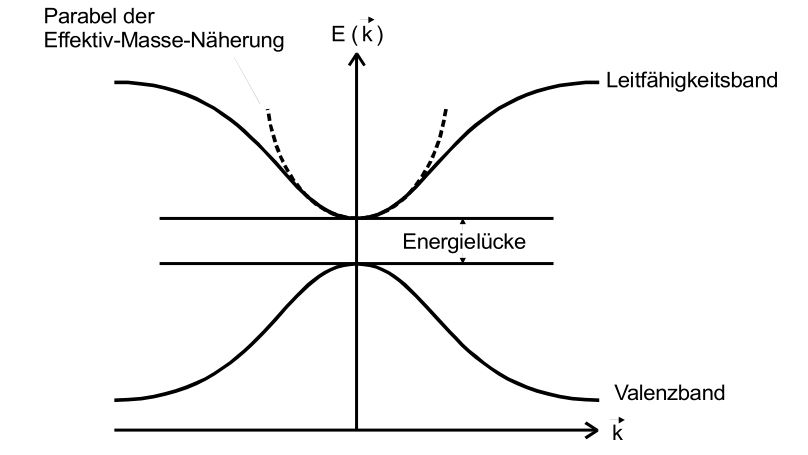
\includegraphics[width=0.5\textwidth]{pics/Energiebaender.jpg}
 \caption{Schematische Darstellung der Bandstruktur eines Festkörpers.\cite{1}}  %?? ändern
 \label{fig:Energiebänder}
 \end{figure}
 An der Stelle $k=0$ lässt sich die Funktion $\epsilon(\vec{k})$, welche die Elektronenenergie beschreibt, um ihr Minimum entwickeln.
 \begin{equation}
   \epsilon(\vec{k})= \epsilon(0)+\frac{1}{2}\sum_{i=1}^3\left(\frac{\partial^2 \epsilon}{\partial{k_i}^2}\right)|_{k=0}{k_i}^2+...
   \label{eq:TaylorEnergie}
 \end{equation}
 Mit
 \begin{equation}
   \epsilon = \frac{\hbar^2 k^2}{2m}
   \label{eq:Epsilonausdruck}
 \end{equation}
 lässt sich \ref{eq:TaylorEnergie} zu einer Ellipsoidgleichung umstellen,
  welche die Flächen gleicher Energien im $\vec{k}-$Raum beschreibt.\\
  Für hohe Symmetrien erhält man Kugelförmige Energieflächen
  \begin{equation}
    \epsilon(\vec{k})= \epsilon(0)+\frac{\hbar^2 k^2}{2m*}.
   \label{eq:KugelEnergie}
  \end{equation}
 Das $m*$ beschreibt hierbei die effektive Masse eines Kristallelektrons mit
 \begin{equation}
   m*:=\frac{\hbar^2}{\left(\frac{\partial^2 \epsilon}{\partial{k_i}^2}\right)|_{k=0}} .
 \end{equation}
 Diese Definition hat den Vorteil, dass die Elektronen eines Kristall mit hoher Symmetrie durch die Bewegungsgleichung
 freier Teilchen beschrieben werden können. In einem periodischen Kristallpotential $V(\vec{r}+\vec{g})$ gilt
  also durch das Einführen der effektiven Masse für den Hamilton-Operator
 \begin{equation}
   \mathcal{H}=\frac{\hbar^2}{2m*}\Delta
   \label{eq:freiHamilton}
 \end{equation}
 \subsection{Rotation der Polarisationsebene}
  Das Phänomen der Drehung der Polarisationsebene eines, durch einen Kristall fallenden linear
  polarisierten Lichtstrahls nennt man
  zirkuläre Doppelbrechnung.\\
  Dies kann durch die Annahme unterschiedlicher Phasengeschwindigkeiten für rechts- und
   linkspolarisiertes Licht im Kristall erklärt werden.\\
  Wird eine elektromagnetische Welle $E(z)$ in zwei unterschiedlich polarsierte Wellen zerlegt, die sich beide in $z$-Richtung
  ausbreiten aber unterschiedliche Wellenzahlen besitzen, kann die Welle durch
  \begin{equation}
    E(z)=\frac{1}{2}\left(E_{\text{R}}(z)+E_\text{{L}}(z)\right), \hspace{2cm}\text{mit} k_{\text{R}} \neq  k_{\text{L}}
    \label{eq:Wellezerlegt}
  \end{equation}
  beschrieben werden.\\
  Damit lässt sich der Winkel, um den die Polarisationsebene des Lichtstrahls rotiert wurde,
  nachdem er den Kristall der Länge $L$ durchquert hat, mit
  \begin{align}
    \theta &=\frac{L}{2} \left(k_{\text{R}}-k_{\text{L}}\right)\\
          &=\frac{L\omega}{2}\left(\frac{1}{v_{\text{ph}_{\text{R}}}}-\frac{1}{v_{\text{ph}_{\text{L}}}}\right)\\
          &=\frac{L\omega}{2\text{c}}\left(n_{\text{R}}-n_{\text{L}}\right)
  \end{align}
  beschreiben. Wobei $v_{\text{ph}}=\frac{\omega}{k}$ die Phasengeschwindigkeit $n=\frac{c}{v_{\text{ph}}}$ der Brechungsindex ist.\\
  Die Doppelbrechung entsteht durch elektrische Dipolmomente, welche pro Volumen eine Polarisation
  \begin{equation}
    \vec{P}=\epsilon_0 \chi \vec{E}
  \end{equation}
  erzeugt.\\
  Die elektrische Suszeptibilität $\chi$ wird hierbei durch einen Tensor beschrieben.
  Dieser hat für doppeltberechende Materie die Form
  \begin{equation}
    \left( \chi \right)=
    \begin{pmatrix}
      \chi_{\text{xx}} & i\chi_{\text{xy}} & 0 \\
      -i \chi_{\text{xy}}& \chi_{\text{xx}} & 0 \\
      0& 0 & \chi_{\text{zz}}
      \end{pmatrix} .
    \end{equation}
  Unter Verwendung der Wellengleichung lässt sich zeigen, dass der Drehwinkel durch
  \begin{equation}
    \theta=\frac{L\omega}{2\text{c}n}\chi_{\text{xy}}
  \end{equation}
  gegeben ist.\\
  Um die Komponente $\chi_{\text{xy}}$ zu bestimmen, wird die Bewegungsgleichung
  eines gebundendes Elektron betrachtet.
  \begin{equation}
    m\frac{\text{d}^2 \vec{r}}{\text{dt}^2}+K\vec{r}= -\text{e}_0
    \vec{E}(r)-\text{e}_0\frac{\text{d}\vec{r}}{\text{dt}}\times \vec{B}
    \end{equation}
  Hierbei werden Dämpfungseffekte vernachlässigt und wegen des hohem $\omega$ wird nur eine
  Verschiebungspolarisation $\vec{P} \propto \vec{r}$ betrachtet.\\
  Damit lässt sich für ein äußeres Magnetfeld in $z$-Richtung zeigen, dass
  die beiden nichtdiagonalelemente komplex konjungiert sind und sich $\theta$ in Abhängigkeit der
  Wellenlänge $\lambda$ durch
  \begin{equation}
    \theta(\lambda)=\frac{2\pi^2 \text{e}_0^3 \text{c}}{\epsilon_0}\frac{1}{m^2 \lambda^2 \omega{_0}^4}\frac{N B L}{n}
    \label{eq:WinkelLambda}
  \end{equation}
      beschreiben lässt.
  Für den Fall von freien Ladungsträgern wird $\omega_0 \rightarrow 0$ betrachtet und es ergibt sich für den Drehwinkel
\begin{equation}
  \theta_{\text{frei}}=\frac{\text{e}_0^3}{8 \pi^2 \epsilon_0 \text{c}^3}\frac{\lambda^2}{m^2}\frac{N L B}{n}
  \label{eq:Winkelfrei}
\end{equation}
\subsection{Durchführung}
Der Aufbau ist in der Grafik \ref{fig:Aufbau} abgebildet.
\begin{figure}[H]
\center
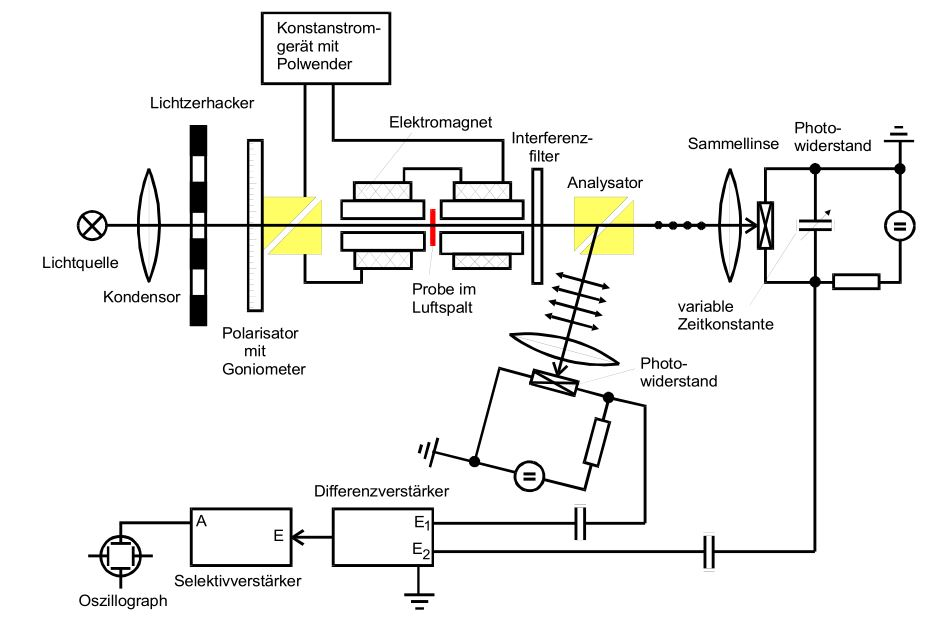
\includegraphics[width=0.5\textwidth]{pics/Aufbau.jpg}
\caption{Schematische Darstellung des Versuchsaufbaus.\cite{1}}  %?? ändern
\label{fig:Aufbau}
\end{figure}
